% Appendix placeholder — add supplementary material here
\section*{Appendix}

\subsection*{A. Additional Figures}

\begin{figure}[h]
\centering
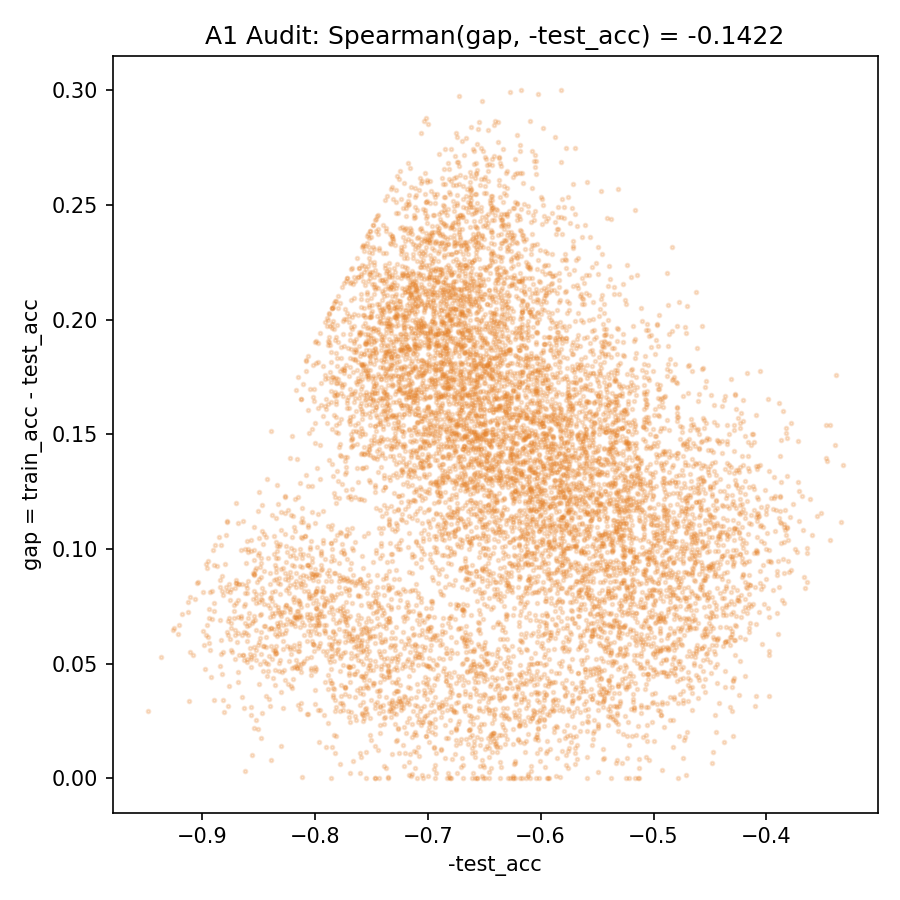
\includegraphics[width=0.9\columnwidth]{figures/a1_audit_scatter}
\caption{A1 audit scatter: gap vs.\ $-$test\_acc. Spearman $= -0.142$, confirming independence.}
\label{fig:a1_audit}
\end{figure}

\begin{figure}[h]
\centering
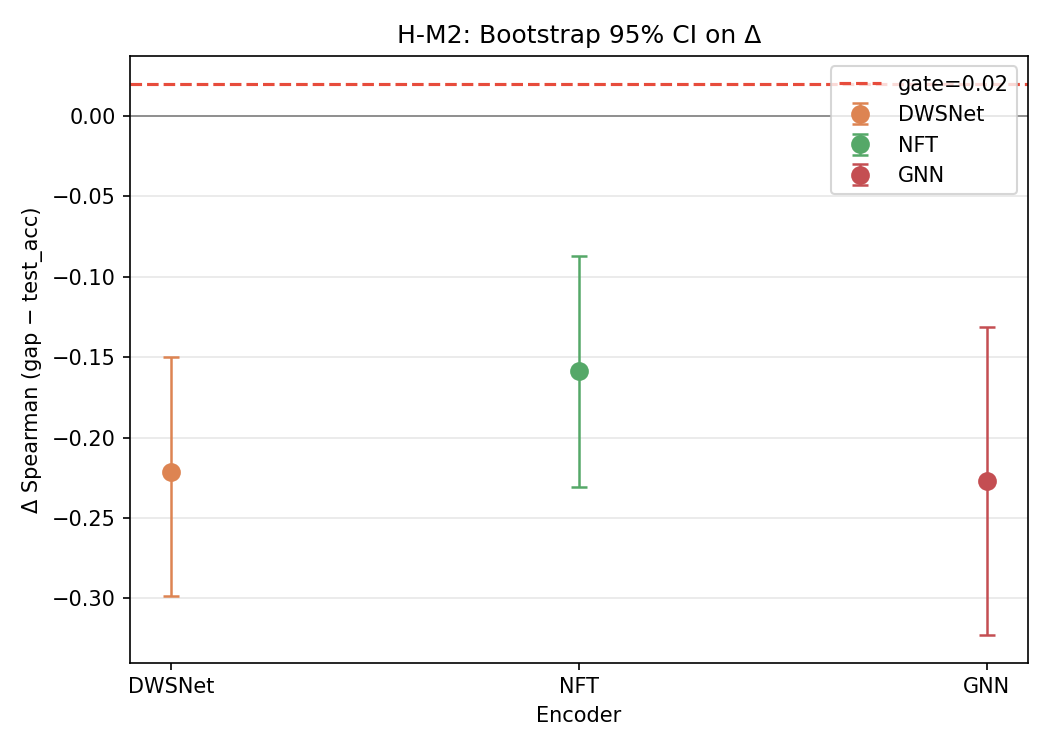
\includegraphics[width=0.9\columnwidth]{figures/fig5_bootstrap_ci}
\caption{Bootstrap 95\% confidence intervals for all Spearman estimates.}
\label{fig:bootstrap_ci}
\end{figure}

\begin{figure}[h]
\centering
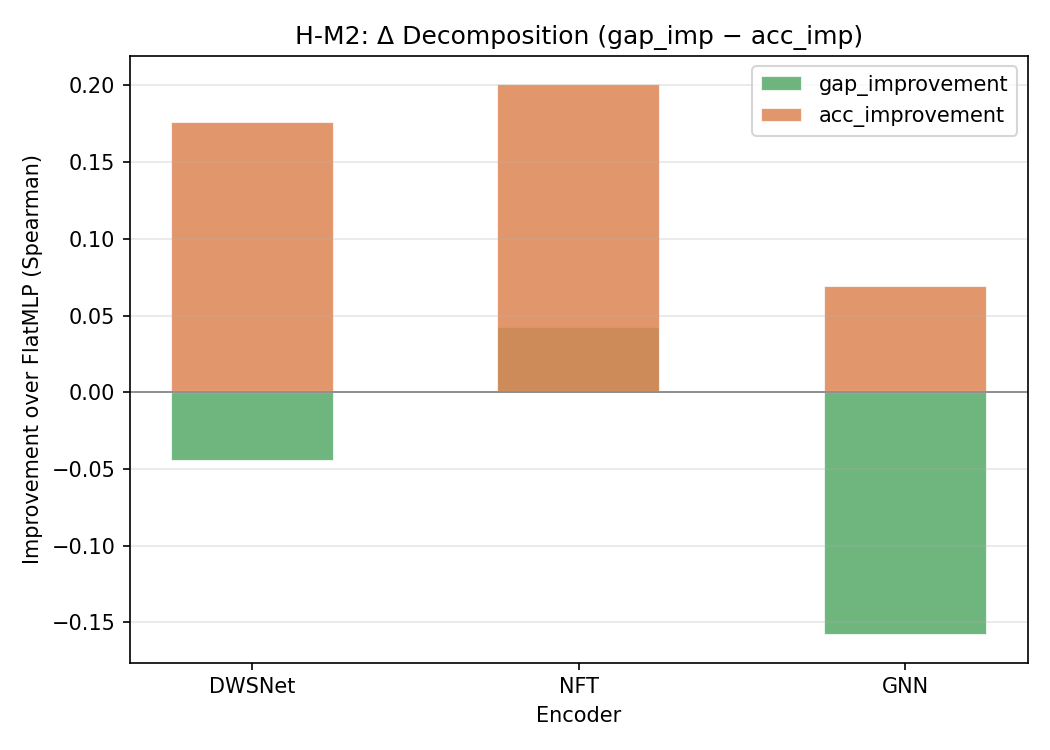
\includegraphics[width=0.9\columnwidth]{figures/fig3_delta_decomposition}
\caption{$\Delta$ decomposition: gap improvement vs.\ test\_acc improvement over FlatMLP for each equivariant encoder.}
\label{fig:delta_decomp}
\end{figure}

\begin{figure}[h]
\centering
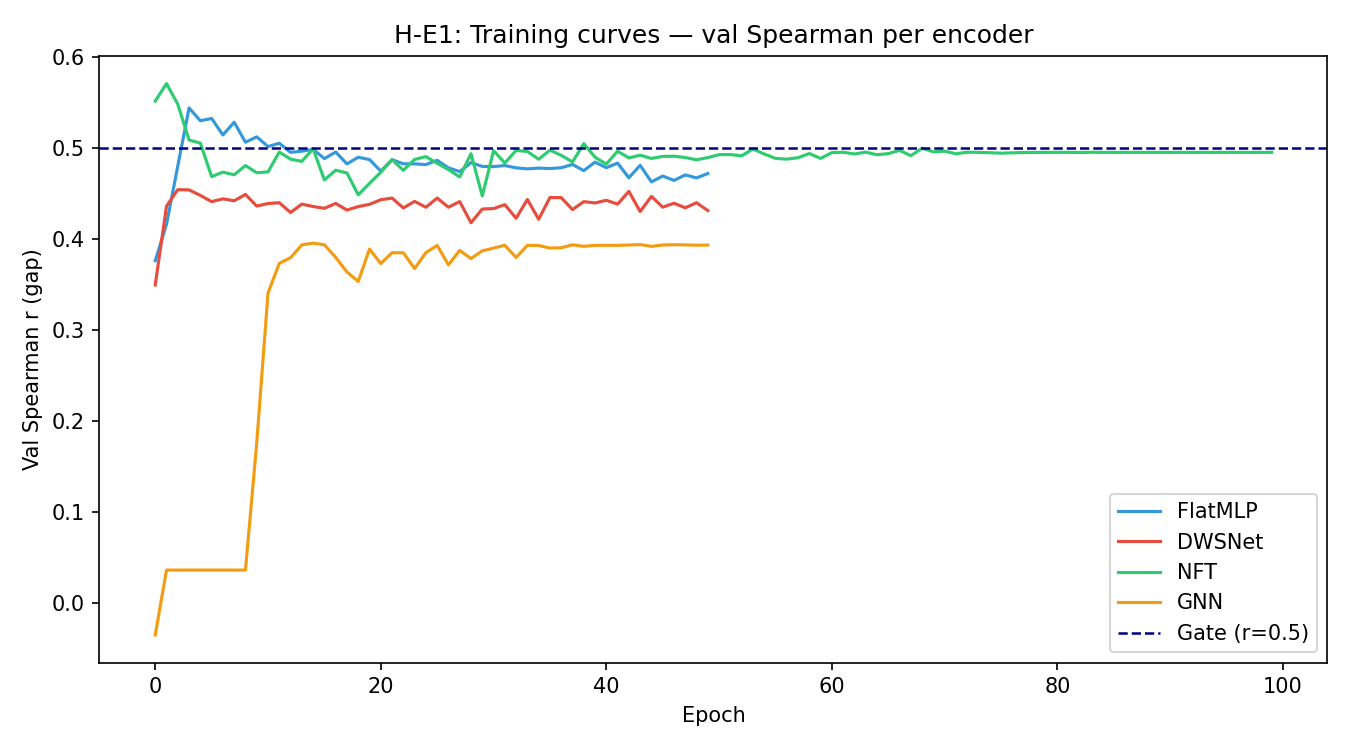
\includegraphics[width=0.9\columnwidth]{figures/training_curves}
\caption{Training curves (validation Spearman vs.\ epoch) for all encoders on both targets.}
\label{fig:training_curves}
\end{figure}
